%% ============================================================================
%%  One Codebook for Every Architecture:
%%  Asymmetric NormalFloat for Calibration-Free KV-Cache Quantization
%%
%%  TMLR submission — Overleaf project root.   Full rewrite, 2026-08-24.
%%
%%  Author actions from REVIEW-2026-08-24.md applied 2026-09-03: official
%%  tmlr.sty/tmlr.bst (JmlrOrg/tmlr-style-file), both perplexity protocols
%%  stated, breadth table rebuilt on corrected arms with provenance in the
%%  caption, metadata overhead recomputed at the harness's group 32 / fp16,
%%  Llama-2-13B resolved to results_matrix.json (17.34).
%%
%%  STYLE: tmlr.sty and tmlr.bst are the official files from
%%  https://github.com/JmlrOrg/tmlr-style-file. Under review the author block
%%  is anonymised by the style; switch to \usepackage[accepted]{tmlr} for the
%%  camera-ready and fill in \month/\year/\openreview below.
%% ============================================================================
\documentclass{article}

\usepackage{tmlr}                 % under review (anonymised by the style)
% \usepackage[accepted]{tmlr}     % camera-ready
% \usepackage[preprint]{tmlr}     % arXiv preprint (de-anonymised, no header)
\def\month{09}
\def\year{2026}
\def\openreview{\url{https://openreview.net/forum?id=XXXX}}

\usepackage{graphicx}
\usepackage{booktabs}
\usepackage{amsmath,amssymb,amsthm}
\usepackage{xcolor}
\usepackage{caption}
\usepackage{subcaption}
\usepackage{microtype}
\usepackage{url}
\usepackage[colorlinks=true,linkcolor=blue,citecolor=blue,urlcolor=blue]{hyperref}
\usepackage[capitalize]{cleveref}
% natbib is loaded by tmlr.sty (author-year, round brackets).

\theoremstyle{plain}
\newtheorem{theorem}{Theorem}
\newtheorem{proposition}[theorem]{Proposition}
\newtheorem{lemma}[theorem]{Lemma}
\theoremstyle{definition}
\newtheorem{definition}[theorem]{Definition}
\newtheorem{remark}[theorem]{Remark}

\captionsetup{font=small,labelfont=bf}
\graphicspath{{figs/}}
\definecolor{collapse}{HTML}{d1495b}
\newcommand{\collapse}[1]{\textcolor{collapse}{\textbf{#1}}}
\newcommand{\absmax}{\mathrm{absmax}}
\newcommand{\NF}{\mathrm{NF4}}
\newcommand{\tr}{\mathrm{tr}}

\title{One Codebook for Every Architecture:\\
       Asymmetric NormalFloat for Calibration-Free KV-Cache Quantization}

\author{\name Andrew H. Bond \email andrew.bond@sjsu.edu \\
  \addr Department of Computer Engineering, San Jos\'e State University}

\begin{document}
\maketitle

\begin{abstract}
Quantizing the key--value (KV) cache is the standard route to long-context LLM inference, and
the data-free NormalFloat-4 (NF4) codebook \citep{dettmers2023qlora} is a popular
calibration-free choice. We show that \textbf{NF4 fails silently and catastrophically on an
entire class of models}---those with high-ratio grouped-query attention
(GQA)~\citep{ainslie2023gqa}---while appearing excellent on the Llama-family
multi-head-attention (MHA) models that dominate published KV-quantization benchmarks. On
Qwen2.5-7B (7:1 GQA), 4-bit NF4 KV quantization collapses LongBench-qasper from \textbf{43.8
(fp16) to 4.7} and WikiText-2 perplexity from \textbf{7.46 to 74.7}---degenerate
repetition---whereas the same recipe is near-lossless on Llama-2-7B/13B and Mistral-7B. We
decompose the failure into two measured factors. \emph{Representation}: KV keys carry a large
per-channel DC offset, so NF4's zero-centred abs-max grid spends about half of its codes where
there is no data---a claim we make exact and machine-check in Lean~4/Mathlib, which also shows
the offset correction is optimal and worth a factor $2/\rho$ in worst-case error. \emph{Error
tolerance}: NF4's key reconstruction error is \emph{equal} on Qwen and Llama, so representation
alone cannot explain the collapse; the high-GQA model routes each KV-head error into seven query
heads and cannot absorb it. Equal error, unequal outcome---the two models differ in how they
\emph{read} the same perturbation. The fix follows from the decomposition: \textbf{asymmetric
NF4 (asym-NF4)} adds a single per-channel zero-point, and is near-fp16 on \emph{every}
architecture we test, recovering the Qwen collapse to \textbf{41.9 qasper / 7.50 ppl} at an
11\% metadata overhead (one extra fp16 scalar per 32-element group). We further show the offset is \emph{RoPE-frequency-structured},
yielding a zero-point computable from weights and configuration alone---calibration-free in the
strict sense---that matches calibrated asym-NF4. We release the method, a reproducible
cross-model harness, the Lean development, and a practitioner's decision guide.
\end{abstract}

\section{Introduction}
The KV cache dominates the memory footprint of long-context inference~\citep{kwon2023vllm}, and
4-bit quantization of keys and values is now standard practice. Calibration-free codebooks are
attractive because they require no data pass and no stored statistics: the 4-bit NormalFloat
(NF4) grid, popularised by QLoRA~\citep{dettmers2023qlora}, allocates levels by a unit Gaussian
and is a common default for KV keys.

Most KV-quantization studies~\citep{hooper2024kvquant,liu2024kivi,zhang2023h2o} benchmark on the
Llama family~\citep{touvron2023llama2}. We show that this practice hides a failure that is both
catastrophic and silent: no exception, no warning, no obviously broken tensor---simply worse
answers, and on one architecture class, degenerate ones.

The paper's organising claim is a decomposition. A quantizer's downstream damage is not a
property of the quantizer alone; it is the product of \emph{how badly the codebook represents
the data} and \emph{how strongly the consumer amplifies the resulting error}. Both factors are
measurable, and separating them is what turns a mysterious collapse into a one-line fix. Our
mechanism section measures each in turn and shows that the first is constant across the models
that survive and the model that collapses---so the second is the whole story.

\paragraph{Contributions.}
\begin{enumerate}
  \item \textbf{A silent, catastrophic failure mode} of NF4 KV quantization on high-GQA models
        (Qwen2.5), invisible on the Llama-family models typically benchmarked
        (\Cref{sec:headline}).
  \item \textbf{A two-factor mechanism, measured}: NF4 costs ${\sim}3$--$5\times$ the relative
        key reconstruction error of asymmetric uniform on DC-offset keys, \emph{equally} on
        Qwen and Llama; the GQA ratio then sets the error tolerance. Bit-depth is not the
        axis---3-bit \emph{uniform} beats 4-bit NF4 on Qwen (\Cref{sec:anatomy}).
  \item \textbf{Machine-checked geometry} (\Cref{sec:formal}): the ``wastes half its codes''
        claim, the optimality of the zero-point, and a $2/\rho$ error-ratio bound are proved in
        Lean~4/Mathlib---12 theorems, no \texttt{sorry}---and hold for any 16-level grid.
  \item \textbf{The offset is RoPE-frequency-structured} (\Cref{sec:rope}), which yields a
        zero-point computable from weights and config alone, with no calibration pass and no
        per-channel metadata, matching calibrated asym-NF4 on perplexity and task score.
  \item \textbf{asym-NF4} (\Cref{sec:method}): a one-line per-channel zero-point that unifies
        the codebook choice across architectures at 11\% metadata overhead.
  \item A reproducible single harness, a cross-model matrix, the Lean development, and a
        practitioner decision guide (\Cref{sec:repro}).
\end{enumerate}

\section{Related work}
\label{sec:related}
\paragraph{Weight and activation quantization.} Post-training quantization of weights is
well developed---GPTQ~\citep{frantar2023gptq}, AWQ~\citep{lin2024awq}---as is the treatment of
activation outliers~\citep{dettmers2022llmint8,xiao2023smoothquant}. NF4 itself originates in
QLoRA's weight quantization~\citep{dettmers2023qlora}, where the unit-Gaussian level allocation
matches weight distributions that are, by construction of the training process, close to
zero-centred. Our finding is in part a statement about \emph{transfer}: the distributional
assumption that makes NF4 excellent for weights does not hold for KV keys, which carry a
systematic per-channel offset (\Cref{sec:rope}).

\paragraph{KV-cache quantization.} KVQuant~\citep{hooper2024kvquant} uses offline
Fisher-weighted non-uniform quantization with per-channel key grids and pre-RoPE quantization;
KIVI~\citep{liu2024kivi} is tuning-free and asymmetric, quantizing keys per channel and values
per token at 2 bits. Both report on Llama-family models. KIVI's asymmetry is the closest prior
art to our fix and we regard our result as an explanation of \emph{why} that design choice
matters more than its authors' evaluation could show: on the MHA models KIVI evaluates, the
symmetric/asymmetric distinction is worth a few points, and on high-GQA models it is the
difference between working and not. Eviction-based methods such as
H2O~\citep{zhang2023h2o} and attention-sink retention~\citep{xiao2024streamingllm} are
orthogonal---they choose \emph{which} entries to keep, not how to encode them---and compose
with our codebook.

\paragraph{Attention geometry.} GQA~\citep{ainslie2023gqa} and its
predecessor MQA~\citep{shazeer2019mqa} reduce KV memory by sharing key/value heads across query
heads. Their cost is normally discussed in terms of model quality at training time. We show
they additionally change a model's \emph{robustness to KV perturbation}, which is a
deployment-time property that the KV-quantization literature has not accounted for.
Rotary embeddings~\citep{su2024roformer} supply the structure behind the offset in
\Cref{sec:rope}.

\section{Background and setup}
\label{sec:setup}
We quantize keys per channel and values per token, with optional dense-and-sparse fp16 outliers
(top 2\% magnitude per channel, following \citealp{dettmers2022llmint8}) and an attention
sink~\citep{xiao2024streamingllm}, in a deployable prefill-once cache that runs at ${\sim}$fp16
speed. We compare four calibration-free key codebooks at 4 bits: fp16 (reference), symmetric
NF4 (abs-max scaling about zero), asymmetric uniform (per-group min/max), and our asym-NF4.

Models span the GQA spectrum: Llama-2-7B/13B (MHA, 1:1)~\citep{touvron2023llama2}, Mistral-7B
(GQA 4:1)~\citep{jiang2023mistral}, Qwen2.5-7B (GQA 7:1)~\citep{qwen2025qwen25}. We evaluate on
the LongBench English subset~\citep{bai2024longbench} and WikiText-2
perplexity~\citep{merity2017pointer}.

\paragraph{Protocol note.}
Two WikiText-2 perplexity protocols appear in this paper and are \emph{not} mutually
comparable. The \textbf{matrix protocol} (\Cref{tab:ppl}; \texttt{kvquant\_matrix/wikitext\_ppl.py})
scores every non-overlapping $2048$-token chunk of the WikiText-2 test split with the full
recipe of \Cref{tab:qasper}: 4-bit keys \emph{and} 4-bit per-token values, group $32$, $2\%$
fp16 outlier channels, $4$ sink tokens, a $128$-token fp16 recent window, the settled region
quantized once. The \textbf{zero-point protocol} (\Cref{sec:rope};
\texttt{benchmarks/deterministic\_zeropoint.py}) isolates the key codebook: three
non-overlapping $512$-token windows, keys quantized at group $32$, values left in fp16, with
the same sink and recent-window handling. Short windows raise absolute perplexity, which is
why Qwen2.5-7B fp16 reads $7.46$ under the first and $9.06$ under the second; every comparison
we draw is made strictly within one protocol, and the LongBench numbers in \Cref{sec:rope} use
the matrix protocol's harness unchanged.

\section{NF4 fails on high-GQA models}
\label{sec:headline}
\Cref{fig:crossover} and \Cref{tab:qasper} give the headline. NF4 is the stronger of the two
naive codebooks on Llama-2-7B/13B and Mistral, but on Qwen2.5-7B it \collapse{collapses} from
43.8 (fp16) to 4.7---near-random, and qualitatively degenerate: the model emits repetitive
fragments rather than answers. Asymmetric uniform never collapses but sacrifices 5--9 qasper
points on the models where NF4 works. asym-NF4 is best-or-tied on three of four models and
within 1.2 points of NF4 on the fourth, while being the only codebook that never collapses.

Perplexity tells the identical story (\Cref{fig:ppl}, \Cref{tab:ppl}): on Qwen, symmetric NF4
perplexity explodes $10\times$ (7.46$\rightarrow$74.7) while asym-NF4 holds at 7.50. That the
two metrics agree matters: perplexity is continuous and task-free, so the collapse is not an
artifact of LongBench's answer matching.

\begin{figure}[t]
\centering
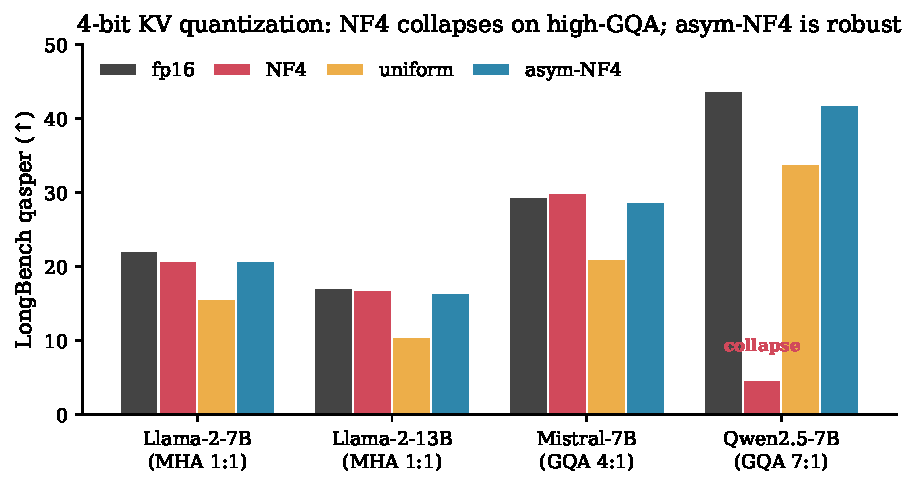
\includegraphics[width=\linewidth]{fig_crossover.pdf}
\caption{4-bit KV quantization on the LongBench qasper task. NF4 (red) is competitive on the
MHA / low-GQA models but \collapse{collapses} on Qwen2.5-7B (7:1 GQA). asym-NF4 (blue) is
near-fp16 on every architecture.}
\label{fig:crossover}
\end{figure}

\begin{table}[t]
\centering\small
\caption{LongBench qasper ($\uparrow$), 4-bit keys, identical outliers/sink. \textbf{Bold}
marks our method, not the per-row maximum; the per-row maximum is \underline{underlined}.
Differences below ${\sim}0.5$ points are within run-to-run variation of this harness.}
\label{tab:qasper}
\begin{tabular}{llrrrr}
\toprule
model & attn (Q:KV) & fp16 & NF4 & uniform & \textbf{asym-NF4} \\
\midrule
Llama-2-7B  & MHA 1:1 & \underline{22.06} & 20.82 & 15.58 & \textbf{20.81} \\
Llama-2-13B & MHA 1:1 & 17.06 & 16.86 & 10.52 & \textbf{\underline{17.34}} \\
Mistral-7B  & GQA 4:1 & \underline{29.43} & 29.96 & 21.06 & \textbf{28.74} \\
Qwen2.5-7B  & GQA 7:1 & \underline{43.77} & \collapse{4.69} & 33.81 & \textbf{41.91} \\
\bottomrule
\end{tabular}
\end{table}

\begin{figure}[t]
\centering
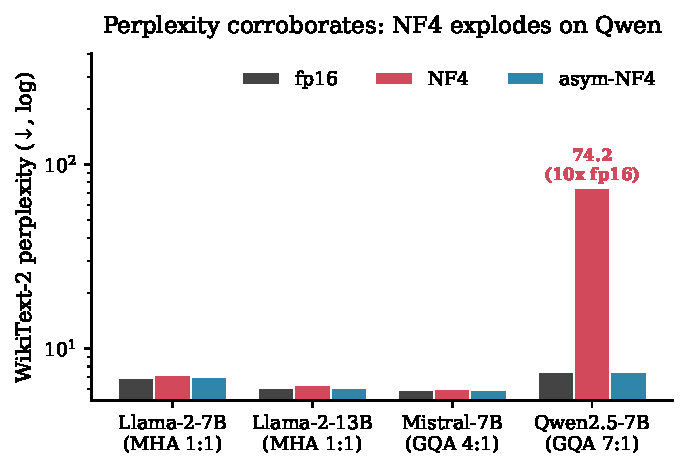
\includegraphics[width=0.72\linewidth]{fig_perplexity.pdf}
\caption{WikiText-2 perplexity ($\downarrow$, log scale). Symmetric NF4 explodes $10\times$ on
Qwen2.5-7B; asym-NF4 sits on fp16 everywhere.}
\label{fig:ppl}
\end{figure}

\begin{table}[t]
\centering\small
\caption{WikiText-2 perplexity ($\downarrow$), same recipe and protocol as \Cref{tab:qasper}.}
\label{tab:ppl}
\begin{tabular}{lrrr}
\toprule
model & fp16 & NF4 & \textbf{asym-NF4} \\
\midrule
Llama-2-7B  & 6.94 & 7.18 & \textbf{6.97} \\
Llama-2-13B & 6.11 & 6.30 & \textbf{6.13} \\
Mistral-7B  & 5.94 & 6.00 & \textbf{5.96} \\
Qwen2.5-7B  & 7.46 & \collapse{74.66} & \textbf{7.50} \\
\bottomrule
\end{tabular}
\end{table}

\section{Anatomy of the collapse: representation \texorpdfstring{$\times$}{x} tolerance}
\label{sec:anatomy}

\paragraph{It is the codebook shape, not the bit-depth.}
\Cref{fig:rescue} isolates the cause on Qwen. Holding the model fixed, 4-bit NF4 scores 4.7;
4-bit \emph{uniform} scores 33.8; and \emph{3-bit} uniform scores 34.9---lower precision,
$7\times$ better. Adding 10\% fp16 outliers, shortening the context, or raising values to 8-bit
all leave NF4 collapsed. Only changing the codebook helps. Whatever is wrong is not a shortage
of bits.

\paragraph{Factor 1: representation.}
On real pre-RoPE keys, NF4 incurs ${\sim}3$--$5\times$ the relative reconstruction error
(whole-key Frobenius) of asymmetric uniform, because KV keys carry a per-group DC offset
(range/abs-max $\approx 0.9$) and NF4's zero-centred grid spends about half of its codes on the
empty side (\Cref{fig:asymnf4}). \Cref{sec:formal} makes both halves of that sentence exact:
a range/abs-max ratio below 1 \emph{entails} one-sided data, and the dead fraction of the grid
span is exactly $(2-\rho)/2 = 0.55$ at the measured $\rho = 0.9$.

\paragraph{Factor 2: tolerance---and it is the whole difference.}
The representation cost above is measured on \emph{both} Qwen and Llama, and it is
\emph{equal} across them (\Cref{fig:mechanism}). This is the pivot of the paper: if the two
models see the same key error and only one collapses, no property of the codebook can explain
the collapse. The differentiator is what the model does with that error. Qwen2.5-7B has 28
query heads and 4 KV heads, so each KV-head perturbation is read by seven query heads;
Llama-2-7B (1:1 MHA) routes it into one. Empirically Qwen collapses above a key-relerr
threshold between 0.04 (uniform-3b) and 0.08 (NF4-4b), while Llama's threshold exceeds 0.08.

\paragraph{Equal error, unequal outcome.}
Stated generally: the damage a quantizer does is not a property of its reconstruction error
alone. It is that error read through the consumer that will use it, and two models with the
same nominal error can sit on opposite sides of a usability cliff. The practical consequence
for evaluation is immediate and, we think, the most transferable claim in this paper: a
reconstruction-error budget calibrated on one architecture does not transfer to another, and a
scalar error target is not a sufficient acceptance test for a KV codebook. A companion
preregistered study on the same model reaches the same conclusion from the opposite
direction---by \emph{equalising} a scalar uncertainty statistic across two structurally
different KV-eviction scorers and finding that decode quality still differed by
$0.359 \pm 0.068$ (5.3 standard errors), the equality prediction it had registered in advance
being refuted \citep{bond2026kvaccess}. Two independent routes, one lesson: match the error
\emph{structure}, not its magnitude.

\begin{figure}[t]
\centering
\begin{subfigure}{0.49\linewidth}\centering
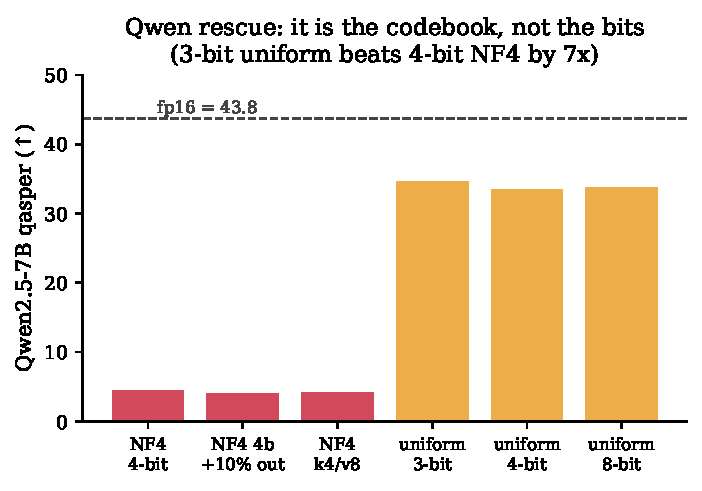
\includegraphics[width=\linewidth]{fig_rescue.pdf}
\caption{Qwen rescue sweep: the codebook, not the bit budget, decides survival.}
\label{fig:rescue}
\end{subfigure}\hfill
\begin{subfigure}{0.49\linewidth}\centering
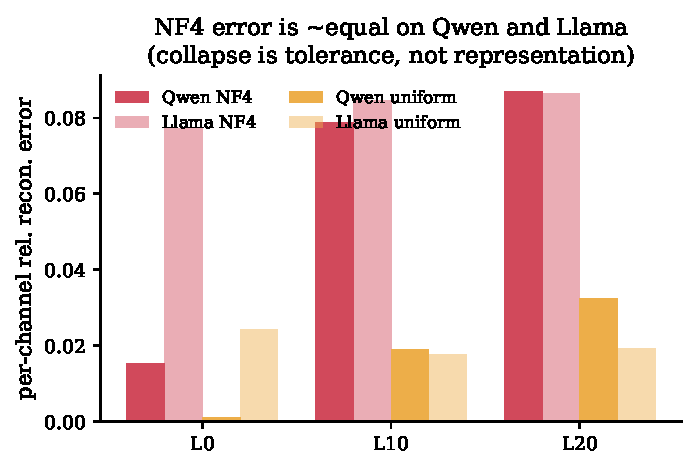
\includegraphics[width=\linewidth]{fig_mechanism.pdf}
\caption{NF4's reconstruction error is ${\sim}$equal on Qwen and Llama: the collapse is error
\emph{tolerance}, not representation.}
\label{fig:mechanism}
\end{subfigure}
\caption{Isolating the two factors behind the Qwen collapse.}
\end{figure}

\section{The geometry, machine-checked}
\label{sec:formal}
Two claims in \Cref{sec:anatomy} are geometric rather than empirical, and we state them as
theorems proved in Lean~4~\citep{demoura2021lean4} against Mathlib~\citep{mathlib2020}. The
development is \texttt{paper/kv\_tmlr/lean/AsymNF4.lean}: 12 theorems, no axioms beyond
Mathlib, no \texttt{sorry}. The statements hold for \emph{any} 16-level grid---they concern
where a grid is \emph{placed}, not how its levels are spaced---so they apply to NF4, to uniform,
and to any other codebook.

Write a channel's data range as $[a,b]$ with $b = \absmax > 0$, and let
$\rho := (b-a)/b$ denote the measured range-to-abs-max ratio.

\begin{theorem}[The diagnostic; \texttt{range\_div\_absmax\_lt\_one}]
\label{thm:diag}
If $0 < a \le b$ then $\rho < 1$; if the data are symmetric about zero ($a = -b$) then
$\rho = 2$. Hence a measured $\rho < 1$ \emph{entails} one-sided data.
\end{theorem}

\begin{theorem}[Wasted codes; \texttt{dead\_code}]
\label{thm:dead}
Let every datum satisfy $x \ge a$ and let $g_1 < g_2 \le a$ be grid points. Then
$|x-g_2| < |x-g_1|$ for every such $x$. No code strictly below the data minimum is ever
emitted.
\end{theorem}

\begin{theorem}[Dead span; \texttt{dead\_span\_fraction}]
\label{thm:span}
For one-sided data on $[a,b]$, a symmetric grid spanning $[-b,b]$ has a dead fraction
$(2-\rho)/2$ of its span. At the measured $\rho = 0.9$ this is $0.55$.
\end{theorem}

\begin{theorem}[Optimality of the zero-point; \texttt{absmax\_sub\_ge\_halfRange}]
\label{thm:opt}
For any offset $c$, $\max(|a-c|,|b-c|) \ge (b-a)/2$, with equality at $c = (a+b)/2$. No offset
achieves a smaller scale than the half-range.
\end{theorem}

\begin{theorem}[Error ratio; \texttt{error\_ratio}]
\label{thm:ratio}
With a common normalized rounding bound $\delta$, the symmetric quantizer (scale $b$) and the
asymmetric one (scale $(b-a)/2$) have worst-case error bounds in ratio $2b/(b-a) = 2/\rho$,
which exceeds $2$ for every strictly one-sided channel and equals $2.22$ at $\rho = 0.9$.
\end{theorem}

\Cref{thm:diag} licenses reading $\rho \approx 0.9$ as evidence of offset rather than as a
heuristic. \Cref{thm:dead,thm:span} make ``wastes half its codes'' exact. \Cref{thm:opt} shows
the zero-point is \emph{optimal}, not merely helpful---no cleverer offset exists.
\Cref{thm:ratio} accounts for a $2.22\times$ error factor from placement alone.

\paragraph{What this does and does not settle.}
The measured ratio is $3$--$5\times$ (\Cref{fig:mechanism}), and the proved bound is
$2.22\times$; the remainder is attributable to NF4's Gaussian level spacing applied to
residuals that are not Gaussian, which these theorems deliberately do not model. Nothing here
bears on Factor 2: the GQA amplification is measured, not proved, and we make no formal claim
about it. We report the decomposition because separating the proved part from the measured part
is more useful than a single unexplained ratio.

\section{Where the offset lives: RoPE-frequency structure}
\label{sec:rope}
The per-channel offset that asym-NF4's zero-point absorbs is not an arbitrary per-channel
statistic---it is concentrated in the \emph{slow rotary channels} of
RoPE~\citep{su2024roformer}. Measuring post-RoPE keys over WikiText-2 windows (512 tokens, 8
passages, all layers and KV heads; \texttt{benchmarks/rope\_offset\_frequency.py}), the
per-channel mean magnitude $|\mu_c|$ correlates strongly with the channel's rotary wavelength
$2\pi\,\theta^{2(c\bmod d/2)/d}$: pooled Spearman $0.91$/$0.96$/$0.94$ on Qwen2.5-1.5B/7B/14B
(per-layer median $0.74$--$0.82$), with $99\%$/$99\%$/$98\%$ of the total offset mass in the
channels whose wavelength exceeds the context window ($67\%$ of channels at $\theta{=}10^6$).
The effect crosses model families: Mistral-7B ($\theta{=}10^4$) gives Spearman $0.98$
(per-layer median $0.95$), with $96\%$ of the mass in $52\%$ of channels.

The mechanism is geometric. A rotary channel whose wavelength exceeds the window is
position-near-invariant within it, so any pre-RoPE per-channel mean survives rotation as a DC
component; fast channels average their mean away over positions. The offset is therefore a
structural property of RoPE at the model's $\theta$ and window, not an accident of a particular
checkpoint---which is why it appears at every scale of the Qwen family and, with a different
base, in Mistral.

\paragraph{A zero-point with no calibration at all.}
This structure yields something stronger than a cheap fix: a zero-point computable from weights
and configuration alone. Pushing the model's own \texttt{k\_proj} bias through the
position-averaged rotation gives a per-channel offset requiring no calibration data and no
stored per-channel metadata. It recovers WikiText-2 perplexity $12.533$/$9.179$ on
Qwen2.5-1.5B/7B versus $12.534$/$9.155$ for calibrated asym-NF4 (fp16 $12.234$/$9.057$;
symmetric NF4 $30.96$/$241.3$)---a dead heat with the calibrated zero-point at zero calibration
cost.\footnote{Absolute values here use the zero-point study's protocol and are not comparable
to \Cref{tab:ppl}; see the protocol note in \Cref{sec:setup}.} Restricting calibrated
zero-points to the config-identified long-wavelength channels alone matches dense calibration
($12.484$/$9.150$) with one-third less metadata.

The result holds at the task level. On LongBench-qasper (Qwen2.5-7B, full $200$-sample split,
one harness), the bias-derived zero-point scores $\mathbf{43.36}$ and the config-sparse
zero-point $42.66$, against $42.35$ for calibrated asym-NF4 in the same run (fp16 $43.77$;
symmetric NF4 $4.69$). Both calibration-lean variants match or exceed dense calibration on the
collapse-sensitive task, though at margins ($1.0$ and $0.3$ points) within this harness's
run-to-run variation; we claim parity, not superiority. The bias route applies to models with
key-projection biases (the Qwen family); bias-free models such as Mistral carry their offsets in
hidden-state statistics and keep the calibrated or sparse variants.

\section{Asymmetric NF4}
\label{sec:method}
asym-NF4 adds a per-channel zero-point. For each channel we subtract the mean $\mu$,
NF4-quantize the residual scaled by its abs-max, and add $\mu$ back at decode:
\[
\hat{x} \;=\; \mu \;+\; \absmax(x-\mu)\cdot
\NF\!\left(\frac{x-\mu}{\absmax(x-\mu)}\right),
\]
where $\NF(\cdot)$ denotes nearest-level rounding onto the 16-level NormalFloat grid on
$[-1,1]$ followed by de-quantization. By \Cref{thm:opt} the mean is within a bounded factor of
the optimal offset and the midpoint attains the optimum exactly; we use the mean because it is
what a single streaming pass already computes.

\paragraph{Cost.}
This stores one extra scalar per channel-group beyond NF4's abs-max. Every experiment in this
paper uses the harness's configuration of group size $32$ with fp16 metadata, so symmetric NF4
costs $4 + 16/32 = 4.5$ bits per key element and asym-NF4 costs $4 + 32/32 = 5.0$: compression
of the quantized key region falls from $3.56\times$ to $3.20\times$ against fp16
($7.11\times$ to $6.40\times$ against fp32), an \textbf{11\% relative overhead}. The
overhead halves at group $64$ and halves again at $128$; the fp16 outlier channels and the
recent-token window are common to all arms and excluded from these ratios. \Cref{sec:rope}
removes the stored zero-point altogether for models with key-projection biases, where it is
derived from weights.

asym-NF4 keeps NF4's nonlinear levels (so it beats uniform on the models where level shape
matters) while centring the grid on the data (so it does not collapse where placement matters).
\Cref{fig:asymnf4} shows the intuition; \Cref{sec:formal} proves it.

\begin{figure}[t]
\centering
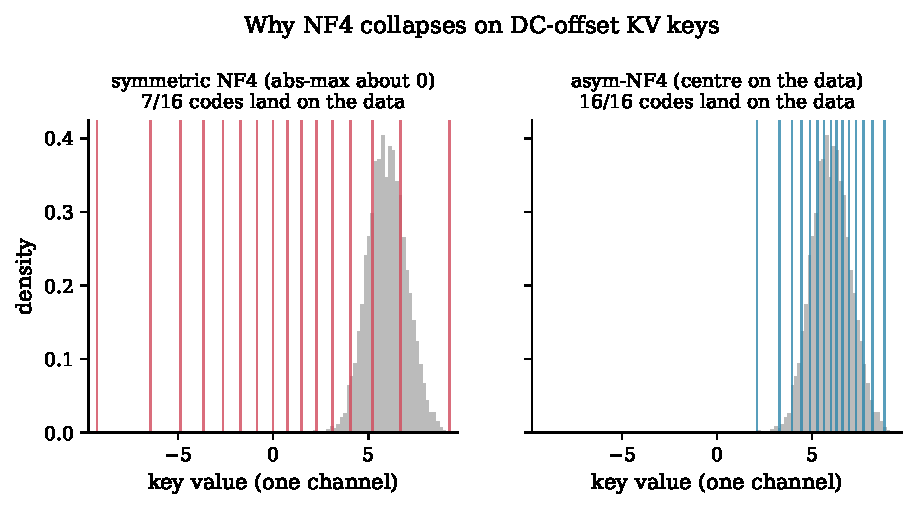
\includegraphics[width=\linewidth]{fig_asymnf4.pdf}
\caption{On a DC-offset key channel, symmetric NF4 (left) places most of its 16 codes where
there is no data; asym-NF4 (right) centres the grid so the codes cover the data.}
\label{fig:asymnf4}
\end{figure}

\paragraph{Breadth.}
\Cref{tab:breadth} extends the Qwen2.5-7B comparison to seven further LongBench tasks
(single- and multi-document QA, multi-hop, summarization, dialogue) spanning generation
lengths from $32$ to $512$ tokens. asym-NF4 is within $1$ point of fp16 on average (mean
gap $0.8$; $41.2 \rightarrow 40.4$), with no task losing more than $1.9$ points as recorded
($3.75$ on 2wikimqa when re-measured at $n{=}40$), and the two long-generation tasks show
\emph{no} residual gap. On the one long-generation cell where symmetric NF4 was re-measured
under the same conditions it scores $5.19$ against fp16 $31.83$---the collapse of
\Cref{sec:headline}, deepening under long decoding.

The table's provenance is deliberately mixed and is stated in the caption: the five
short-generation cells are the recorded full-split values, and the two $512$-token cells are
the $n{=}40$ re-validation values that replaced the retracted record (\Cref{sec:limits}).
An earlier version of this paragraph quoted a 7-task aggregate of $37.3$ for asym-NF4 built on
the retracted cells; that number, and the accompanying claim of a long-generation limitation,
are withdrawn. A single end-to-end re-run of all seven tasks under the harness's config-sidecar
guard is the clean replacement and had not been completed at the time of writing.

\begin{table}[t]
\centering\small
\caption{Qwen2.5-7B, seven further LongBench tasks ($\uparrow$), fp16 vs asym-NF4. Provenance:
the five short-generation rows are the recorded full-split values ($n{=}200$;
\texttt{results\_longgen.json}); the two $512$-token rows are the $n{=}40$ re-validation
values (\texttt{REVAL-2026-08-08}) that replace the retracted record, whose fp16 arm matched
the full-split fp16 to within $0.3$ on both tasks. The 2wikimqa gap re-measured at $3.75$
($n{=}40$) against the recorded $1.9$. Means are over the seven rows as shown.}
\label{tab:breadth}
\begin{tabular}{lrrrr}
\toprule
task & \texttt{max\_gen} & fp16 & asym-NF4 & gap \\
\midrule
2wikimqa            & 32  & 47.1  & 45.2  & 1.9 \\
hotpotqa            & 32  & 57.7  & 56.3  & 1.4 \\
multifieldqa\_en    & 64  & 52.6  & 52.0  & 0.6 \\
narrativeqa         & 128 & 28.8  & 28.1  & 0.7 \\
samsum              & 128 & 46.0  & 45.1  & 0.9 \\
gov\_report ($n{=}40$) & 512 & 31.83 & 32.14 & $-0.31$ \\
multi\_news ($n{=}40$) & 512 & 24.24 & 23.73 & 0.51 \\
\midrule
mean                &     & 41.18 & 40.37 & 0.81 \\
\bottomrule
\end{tabular}
\end{table}

\section{Recommendations}
\label{sec:reco}
Use asym-NF4 by default; in the released library this is
\texttt{TurboQuantKVCache.robust()}. Symmetric NF4 should not be shipped for unknown or
high-GQA models. Asymmetric uniform is a safe but lower-quality fallback. Pre- versus post-RoPE
quantization is a model-specific micro-optimization (it helps Llama-2-7B but hurts Llama-2-13B
and Mistral) and is not a recommended default.

More generally, and independent of our codebook: \textbf{do not accept a KV quantizer on
reconstruction error measured on a different architecture}. \Cref{sec:anatomy} shows the same
error is benign at 1:1 and fatal at 7:1. Acceptance testing should run on the deployment
architecture, and should include at least one task sensitive to degenerate generation---the
Qwen collapse is invisible in a spot check of short answers.

\section{Limitations}
\label{sec:limits}
Four models $\le$13B; LongBench English and WikiText-2; no MoE or $>$13B models. The
GQA-ratio--tolerance hypothesis is tested at four points (1:1, 1:1, 4:1, 7:1), all $\le$13B and
none above 7:1; the mechanism is consistent with the data, but the ratio is not independently
varied within a fixed architecture, which would be the decisive experiment and is future work.

\emph{Same-harness competitor baselines are not yet faithful.} Our in-harness
KVQuant~\citep{hooper2024kvquant} implementation (offline Fisher-weighted per-channel NUQ,
pre-RoPE) runs end to end but reaches only \textbf{8.16} qasper on Llama-2-7B at 4 bits---far
short of the published ${\sim}21$---so it is not a credible reproduction. The KVQuant and
KIVI~\citep{liu2024kivi} comparisons here therefore rest on those papers' published figures
rather than a controlled same-harness run, and a faithful in-harness calibrated comparison
remains future work.

\emph{A retracted result, reported.} An earlier version of this work reported a
long-generation degradation of asym-NF4 (LongBench \texttt{gov\_report} ROUGE falling by 13.7
points at 512 generated tokens, with a monotone sweep across generation lengths). Independent
re-validation using the same harness and LongBench's own metrics
(\texttt{REVAL-2026-08-08}, $n{=}40$) measures a gap of $-0.31$ on that cell; the
\texttt{multi\_news} and Llama-2 rows fail to reproduce identically. The most probable cause is
arm-label contamination during off-repo aggregation of back-to-back \texttt{nf4}/\texttt{nf4a}
sweeps. \textbf{The claim is withdrawn}, and \Cref{tab:breadth} reports the corrected cells. A real and larger long-generation collapse
($26.64$ on the same cell) exists under \emph{symmetric} NF4---that is, it is the collapse of
\Cref{sec:headline} deepening under long decoding, not a codebook-independent limitation. The
harness now rejects unknown codebook identifiers, writes a per-shard config sidecar, and
refuses single-arm aggregation when sidecars disagree.

\section{Reproducibility}
\label{sec:repro}
All results come from a single harness with JSON-recorded numbers and a notebook offering a
single-GPU subset and a multi-GPU full mode (\texttt{benchmarks/kvquant\_matrix/}). Every
reported arm carries a config sidecar naming the codebook actually executed, and the aggregator
refuses to report an arm whose sidecars disagree. The Lean development of \Cref{sec:formal}
builds against Mathlib with no \texttt{sorry}.

\bibliographystyle{tmlr}
\bibliography{references}

\end{document}
